\chapter{Wprowadzenie}
\label{cha:introduction}



%----------------------------------------------------------------------------------------
% Rozbudować
% - tu są tylko główne myśli
% - 
%----------------------------------------------------------------------------------------
\section{Słowo wstępne}

Umiejętność programowania architektur równoległych jest w~dzisiejszych czasach bardzo pożądana. 
Z~przyczyn technologicznych maksymalne taktowanie procesorów sekwencyjnych zatrzymało się na ok. 5 GHz, przy czym praktycznie stosuje się rozwiązania o~taktowaniu mniejszym od 4 GHz.
Zatem postawiono na równoległość. 
Przykładem są procesory wielordzeniowe (CPU -- ang. \textit{Central Processor Unit}, GPP -- ang. \textit{General Purpose Processor}), programowalne karty graficzne (GPGPU --ang. \textit{General-purpose computing on Graphics Processing Units}), a~także rozwiązania hybrydowe łączące obie architektury (np. procesory serii A firmy AMD).
Przy czym jakoś tak dziwnie się składa, że o~ile ludzki mózg działa w~sposób bardzo równoległy (na razie nieosiągalny dla systemów technicznych), to myśleć wolimy w~sposób sekwencyjny.
Programowanie w~klasycznych językach C/C++/C\#/Java/Python stało się wiedzą powszechną i~jest nauczane na wielu różnych szczeblach i kierunkach edukacji. 
Sekwencyjnie podejście jest bardzo intuicyjne i~opisany w ten sposób algorytm łatwo jest zaimplementować.
Z~programowaniem równoległym sprawa wygląda inaczej. 
Wymaga ono innego, chyba znacznie mniej oczywistego, sposobu myślenia.
Przykładowo, na algorytm nie patrzy się jak na "sekwencję instrukcji", ale na "zbiór elementów obliczeniowych" przez które "przepływa" strumień danych.
Ponadto, aby  wykorzystać możliwości jakie oferuje równoległość należy dość dobrze znać wykorzystywaną platformę sprzętową (np. GPU).
W~przypadku programowania na CPU nie ma to tak dużego znaczenia, bo dostępne kompilatory tworzą bardzo dobry kod maszynowy w~sposób automatyczny.
Można wręcz zaryzykować stwierdzenie, że można pisać programy np. w Javie zupełnie nie wiedząc jak działa system komputerowy, procesor itp.

%taksonomia flynna

Programowanie równoległe jest niewątpliwie trudniejsze od sekwencyjnego. 
Jednak wydaje się być na chwilę obecną koniecznością.
Warto zaznaczyć, że wykształcenie umiejętności programowania równoległego, myślenia w kategoriach równoległości jest niezależne od platformy sprzętowej.
Za każdym razem na wejściu mamy algorytm, który chcemy/musimy z~jakiś powodów zrealizować w~sposób równoległy. 
Zmieniają się jedynie narzędzia i architektura, ale idea pozostaje taka sama.

W~ramach niniejszego kursu zajmować się będziemy układami rekonfigurowalnymi (reprogramowalnymi) FPGA (ang. \textit{Field Programmable Gate Array}) -- rozdział \ref{sec:FPGA_SP6}. 
Oprócz tego, że są wręcz idealną platformą do realizacji obliczeń równoległych, to nie mają one zdefiniowanej na etapie produkcji funkcjonal6ności.
Określenie jak będzie działał układ należy do projektanta logiki.
Zatem "programowanie" 
\footnote{w~dalszej części skryptu używane będzie pojęcie \textbf{projektowanie struktury układów FPGA} dla podkreślenia różnic pomiędzy implementacją algorytmu na platformach CPU/GPU, a~FPGA}
układów FPGA różni się od programowania CPU/GPU.
W~pierwszym przypadku budujemy logikę (elementy obliczeniowe oraz pamiętające) z~podstawowych elementów logicznych (bramek, elementów LUT, przerzutników). 
Musimy też określić sposób przepływu danych pomiędzy poszczególnymi modułami.
W~drugim, architekturę mamy ściśle określoną. 
Nasza rola ogranicza się tylko do utworzenia odpowiedniego zbioru instrukcji.

Nauka umiejętności projektowania logiki realizującej jakieś zadania obliczeniowe, najlepiej w sposób mocno równoległy, stanowić będzie "motto" kursu.
W~jego trakcie będziemy często odwoływać się do przykładów i~aplikacji związanych z przetwarzaniem i analizą strumienia wideo, gdyż jest to jedna z dziedzin, gdzie układy FPGA są chętnie stosowane i~mają realną przewagę nad innymi rozwiązaniami \ref{cha:pipelineimageprocessing}. %TODO sprawdzić link
Zadanie jakie stoi przed nami nie jest najłatwiejsze, ale pozwala w~odmienny sposób spojrzeć na "programowanie", co jest bardzo rozwijające.
 
 

%----------------------------------------------------------------------------------------
% Rys historyczny
% - moża historię o językach programowania rozbudować
% - geneza - opis funkcjonanlości, a dopiero później synteza
%----------------------------------------------------------------------------------------
\section{Od lampy elektronowej do układu FPGA -- rys historyczny}

Zasada działania większości maszyn cyfrowych jest podobna. 
Wykorzystują one odpowiednio połączone podstawowe elementy takie jak bramki logiczne (element realizujący obliczenia) i rejestry (element pamiętający) w~celu realizacji bardziej złożonych funkcji. 
W~pierwszych komputerach wykorzystywano przekaźniki i~lampy elektronowe. 
Wraz z rozwojem elektroniki zastosowano tranzystory, a~później układy scalone. 
Te ostatnie ulegały miniaturyzacji -- od dużych obudów, które zawierały kilka bramek logicznych, po nowoczesne procesory wykorzystywane w~aplikacjach mobilnych, które charakteryzują się niskim zużyciem energii i~dużą wydajnością obliczeniową.

Ten spektakularny rozwój nie byłby możliwy, gdyby nie odpowiednie narzędzia, które umożliwiały projektowanie coraz bardziej skomplikowanych architektur. 
W~latach 80 powstał problem opisu struktury i~zachowania układów scalonych. 
Ciągła miniaturyzacja wymuszała tworzenie coraz bardziej skomplikowanych struktur, natomiast wykorzystywane metody projektowania układów przy pomocy schematu ideowego nie pozwalały na osiągniecie tego celu w~prosty sposób. 
W związku z~tym, powstało zapotrzebowanie na tzw. język opisu sprzętu (HDL ang. \textit{Hardware Description Language}). 
Jednym z~lepiej znanych jest opracowany w latach 80 przez Departament Obrony Stanów Zjednoczonych język VHDL (ang. \textit{Very High Speed Integrated Circuits Hardware Description Language}). 

Języki opisu sprzętu miały szereg zalet w~stosunku do schematów ideowych. 
Po pierwsze pozwalały na łatwe wykorzystanie poprzednio stworzonych systemów w~nowych rozwiązaniach. 
Po drugie szybko zaproponowano narzędzia, które na podstawie opisu na wyższym poziomie pozwalały na stworzenie rzeczywistej struktury układu cyfrowego (na poziomie tranzystorów). 
Zauważono również, że zapis struktury i~zachowania układów cyfrowych przy pomocy języka umożliwia weryfikację i~symulację powstałego rozwiązania. 
Cechy te okazały się bardzo ważne i~przesądziły o~sukcesie języków opisu sprzętu. 
Pozwalały one ograniczyć czas wymagany na tworzenie nowych układów częściowo opartych o~poprzednie rozwiązania. 
Poza tym, symulacja umożliwiała usunięcie wielu wad, bez konieczności długotrwałego i~kosztownego procesu produkcji i~testowania prototypowych układów scalonych. 

%----------------------------------------------------------------------------------------
% Budowa układów FPGA serii Spartan 6 firmy Xilix
% - ryzyko autoplagiatu (TK - phd)
%----------------------------------------------------------------------------------------
\section{Budowa układów FPGA serii Spartan 6 firmy Xilinx}
\label{sec:FPGA_SP6}

Jak już zostało wspominane, aby dobrze projektować logikę dla układów FPGA należy poznać podstawy ich budowy.
W~niniejszym rozdziale zostaną zatem omówione podstawowe zasoby logiczne dostępne w układach Spartan~6 firmy Xilinx.
Ogólny opis rodziny Spartan 6 można odnaleźć w dokumencie \cite{xilix_sp6ugCLB}.

\subsection{Blok CLB}

Podstawowym elementem, z~którego zbudowany jest układ FPGA, to blok CLB (ang. \textit{Configurable Logic Block}). 
Złożony on jest z~dwóch elementów \textit{Slice} i~połączony bezpośrednio z~matrycą przełączeń (ang. \textit{Switch Matrix}). 
Zostało to pokazane na rysunku \ref{fig:fpga_clb}. 
Widoczne linie CIN i~COUT, to szybka logika przeniesienia, wykorzystywana przy realizacji operacji arytmetycznych. 

\begin{figure}[!htb]
\label{fig:fpga_clb}
\centerline{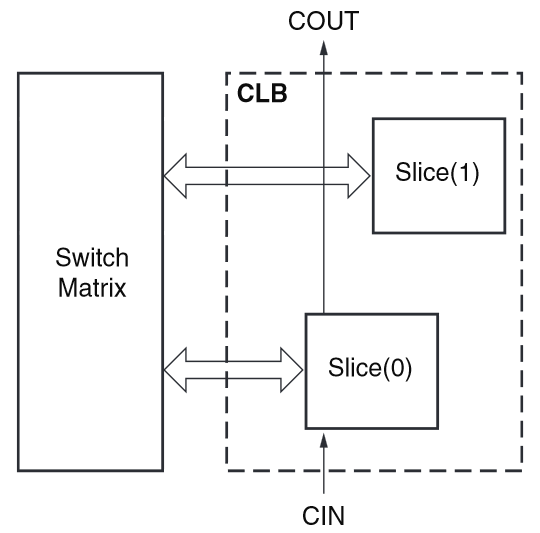
\includegraphics[width=8cm]{introduction/images/fpga_clb}}
\caption{Schemat budowy bloku CLB. Źródło: \cite{xilix_sp6ugCLB}}
\end{figure}

W~układzie Spartan~6 występują trzy rodzaje slice'ów: SLICEX, SLICEL, SLICEM (odpowiednio 50\%, 25\%, 25\% wszystkich w układzie). 
Schemat budowy pojedynczego \textit{slice'u} typu M~zamieszczono na rysunku \ref{fig:fpga_slice}. 

\begin{figure}[!htb]
\label{fig:fpga_slice}
\centerline{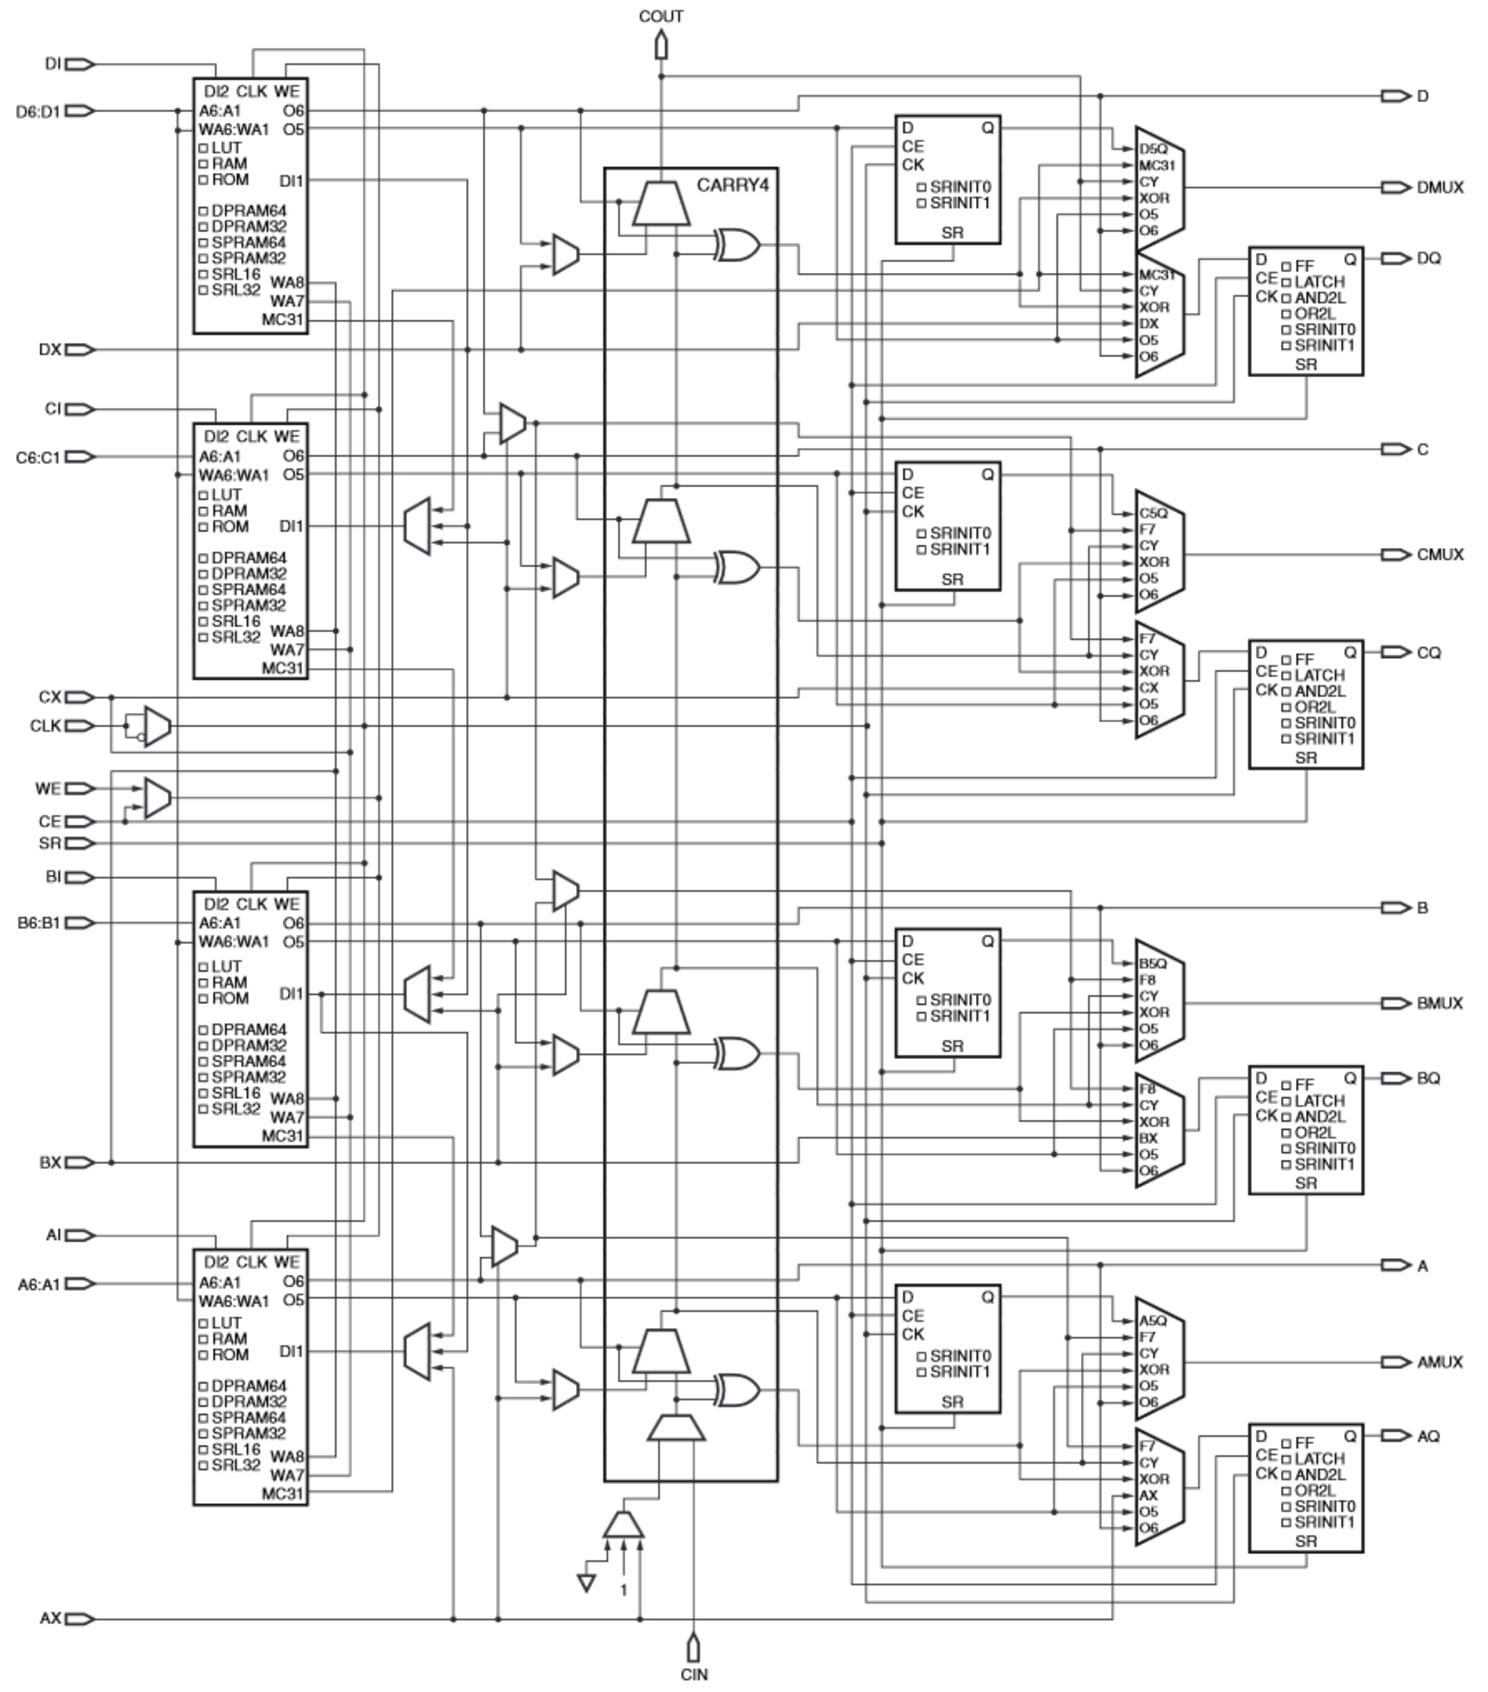
\includegraphics[width=12cm]{introduction/images/fpga_slice}}
\caption{Schemat budowy slice'u typu M.  Z lewej cztery elementy LUT, pośrodku szybka logika przeniesienia, po prawej przerzutniki (4+4) oraz multipleksery. Źródło: \cite{xilix_sp6ugCLB}}
\end{figure}


Złożony on jest z~następujących elementów:
\begin{itemize}
\item generator funkcyjny (4 sztuki) --- został zrealizowany jako {LUT} (ang. \textit{look-up table}) posiadający 6~wejść i~dwa niezależne wyjścia. 
Zatem możliwe jest zaimplementowanie: 6-wejściowej funkcji logicznej, dwóch 5-wejściowych funkcji logicznych (ze~wspólnym wejściem), dwóch funkcji logicznych z~3 i~2 wejściami. 
Ponadto multipleksery umożliwiają tworzenie funkcji 7- i 8-wejściowych poprzez łączenie elementów LUT (SLICEL i~SLICEM). 
Generator funkcyjny może zostać też skonfigurowany jako (tylko SLICEM): 
\begin{itemize}
\item synchroniczna pamięć RAM, zwana pamięcią rozproszoną (ang. \textit{Distributed RAM})
 --- o~różnym rozmiarze i liczbie portów (256 $\times$ 1 jednoportowa, 128 $\times$ 1 dwuportowa i 64 $\times$ 1 czteroportowa), przy czym jeden port umożliwia synchroniczny zapis i~asynchroniczny odczyt, a~pozostałe asynchroniczny odczyt,
\item 32-bitowy rejestr przesuwny wykorzystywany przy tworzeniu linii opóźniających.
\end{itemize}
\item przerzutnik typu D ({FF} --- ang. \textit{Flip-Flop}) --- 8 sztuk), z czego 4 mogą zostać skonfigurowane jako przerzutnik typu D lub zatrzask (ang. \textit{latch}), a~4 tylko jako przerzutnik D,
\item multipleksery --- do łączenia elementów LUT (tylko SLICEL i~SLICEM),
\item szybka logika przeniesienia --- wykorzystywana przy realizacji operacji arytmetycznych.

\end{itemize}

Bardziej szczegółowe informacje dostępne są w dokumencie \cite{xilix_sp6ugCLB} na stronie \texttt{www.xilinx.com}.


\subsection{Pozostałe zasoby}
  
Wśród pozostałych zasobów dostępnych w~układzie FPGA Spartan~6 warto wymienić:
\begin{itemize}
\item {CMT} (ang. \textit{Clock Managment Tiles}) --- bloki zarządzania sygnałem zegarowym, które zapewniają generację różnych częstotliwości zegara, równomierną propagację sygnału zegarowego oraz tłumienie zjawiska \textit{jitter} (zakłócenia fazy zegara). W~układzie znajduje się od 2 do 6 tego typu modułów. Szczegółowe informacje dostępne w dokumencie \cite{xilix_sp6ugCLK},
\item Block RAM (BRAM) --- bloki dedykowanej dwuportowej pamięci RAM o~rozmiarze 18 Kb, które mogą zostać również skonfigurowane jako moduły FIFO. Dostępny rozmiar pamięci w~zakresie od 216 Kb do 4824 Kb.  Szczegółowe informacje dostępne w~dokumencie \cite{xilix_sp6ugBRAM},
\item DSP48A1 --- moduły z~mnożarką 18 $\times$ 18 bitów oraz 48-bitowym akumulatorem. Ich liczba waha się od 9 do 180 w zależności od rozmiaru układu. Szczegółowe informacje dostępne w~dokumencie \cite{xilix_sp6ugDSP},  
\item Select I/O --- zasoby wejścia/wyjścia, podzielone na banki (liczba banków zależy od typu, rozmiaru i obudowy układu i~waha się od 102 do 576 końcówek). Mogą zostać skonfigurowane do pracy z~wieloma standardami (pojedynczymi i różnicowymi): LVCMOS, LVTTL, HSTL, PCI, SSTL, LVDS i~innym. Szczegółowe informacje dostępne w~dokumencie \cite{xilix_sp6ugIO},
\item GTP Transceivers --- moduły nadawczo-odbiorcze umożliwiające szybką transmisją szeregową z~prędkością do 3,2 Gb/s. Wykorzystywane w interfejsach: Serial ATA, Aurora, 1G Ethernet, PCI Express i~innych. Ich liczba waha się od 0 do 8. Nie występują we wszystkich układach z~rodziny Spartan 6. Szczegółowe informacje dostępne w dokumencie \cite{xilix_sp6ugGTP},
\item Zintegrowany moduł PCI Express --- wspiera transmisję z~przepustowością 2,5 Gb/s w~standardzie PCI Express 1.1. Nie występuje we wszystkich układach z~rodziny Spartan 6. Szczegółowe informacje dostępne w dokumentach \cite{xilix_sp6ugPCI} i~\cite{xilix_sp6ugPCIAXI},
\item Zintegrowane kontrolery zewnętrznej pamięci RAM --- moduły stanowiące kontrolery dla pamięci DDR, DDR2, DDR3 oraz LPDDR. Obsługują transmisję do 800 Mb/s oraz umożliwiają tworzenie dostępów wieloportowych. Ich liczba waha się od 0 do 4. Nie występują we wszystkich układach z~rodziny Spartan 6. Szczegółowe informacje dostępne w~dokumencie \cite{xilix_sp6ugRAM}  
\end{itemize}

Ponadto warto zwrócić uwagę, że oprócz zasobów logicznych, w~układzie FPGA występuje cały szereg zasobów połączeniowych w~formie linii globalnych i~lokalnych. 
Wyróżnia się linie lokalne o~pojedynczej, podwójnej i poczwórnej długości oraz globalne.
Osobne zasoby połączeniowe służą do dystrybucji sygnału zegarowego.



%TODO - dopisać krótką notatkę o Virtex6, Virtex 7, Kintex 7, Artix 7, UltraScale, 3D IC  Zynq

